\documentclass[usletter, 10pt, conference]{ieeeconf}
\newcommand{\mbm}[1]{\mbox{\boldmath $#1$}}
\newcommand{\norm}[1]{\lVert#1\rVert}
\newcommand{\superscript}[1]{\ensuremath{^{\textrm{#1}}}}
\newcommand\blfootnote[1]{%
  \begingroup
  \renewcommand\thefootnote{}\footnote{#1}%
  \addtocounter{footnote}{-1}%
  \endgroup
}
\usepackage{url}

\usepackage[ruled,noend,linesnumbered]{algorithm2e}
\usepackage{subfigure}
\usepackage{graphicx,color,psfrag}
\usepackage{amsmath}
\usepackage{amsfonts}
\usepackage{amssymb}
\usepackage{bigdelim}
\usepackage{dsfont}
\usepackage{color, soul}
%\usepackage[section]{placeins}
%\usepackage{graphicx}
%\usepackage{caption}
%\usepackage{subcaption}

\pdfminorversion=4
\IEEEoverridecommandlockouts                              
\overrideIEEEmargins

\newcommand{\ville}[1]{\textcolor{blue}{\small Ville: #1}}
\newcommand{\raj}[1]{\textcolor{green}{\small Raj: #1}}

\title{Semantic-MultiKinFu: Multiple Semantic-TSDF 3D grid Maps for Warehouse Robots} 

% Multiple authors
\author{Dinh-Cuong Hoang$^{*}$, Todor Stoyanov$^{*}$, and Achim J. Lilienthal$^{*}$% <-this % stops a space
\thanks{*Centre for Applied Autonomous Sensor Systems (AASS); Orebro University.}% <-this % stops a space
}

\begin{document}
\maketitle
\thispagestyle{empty}
\pagestyle{empty}
%
%

\begin{figure*}[t!]
\centering
\subfigure[] {
        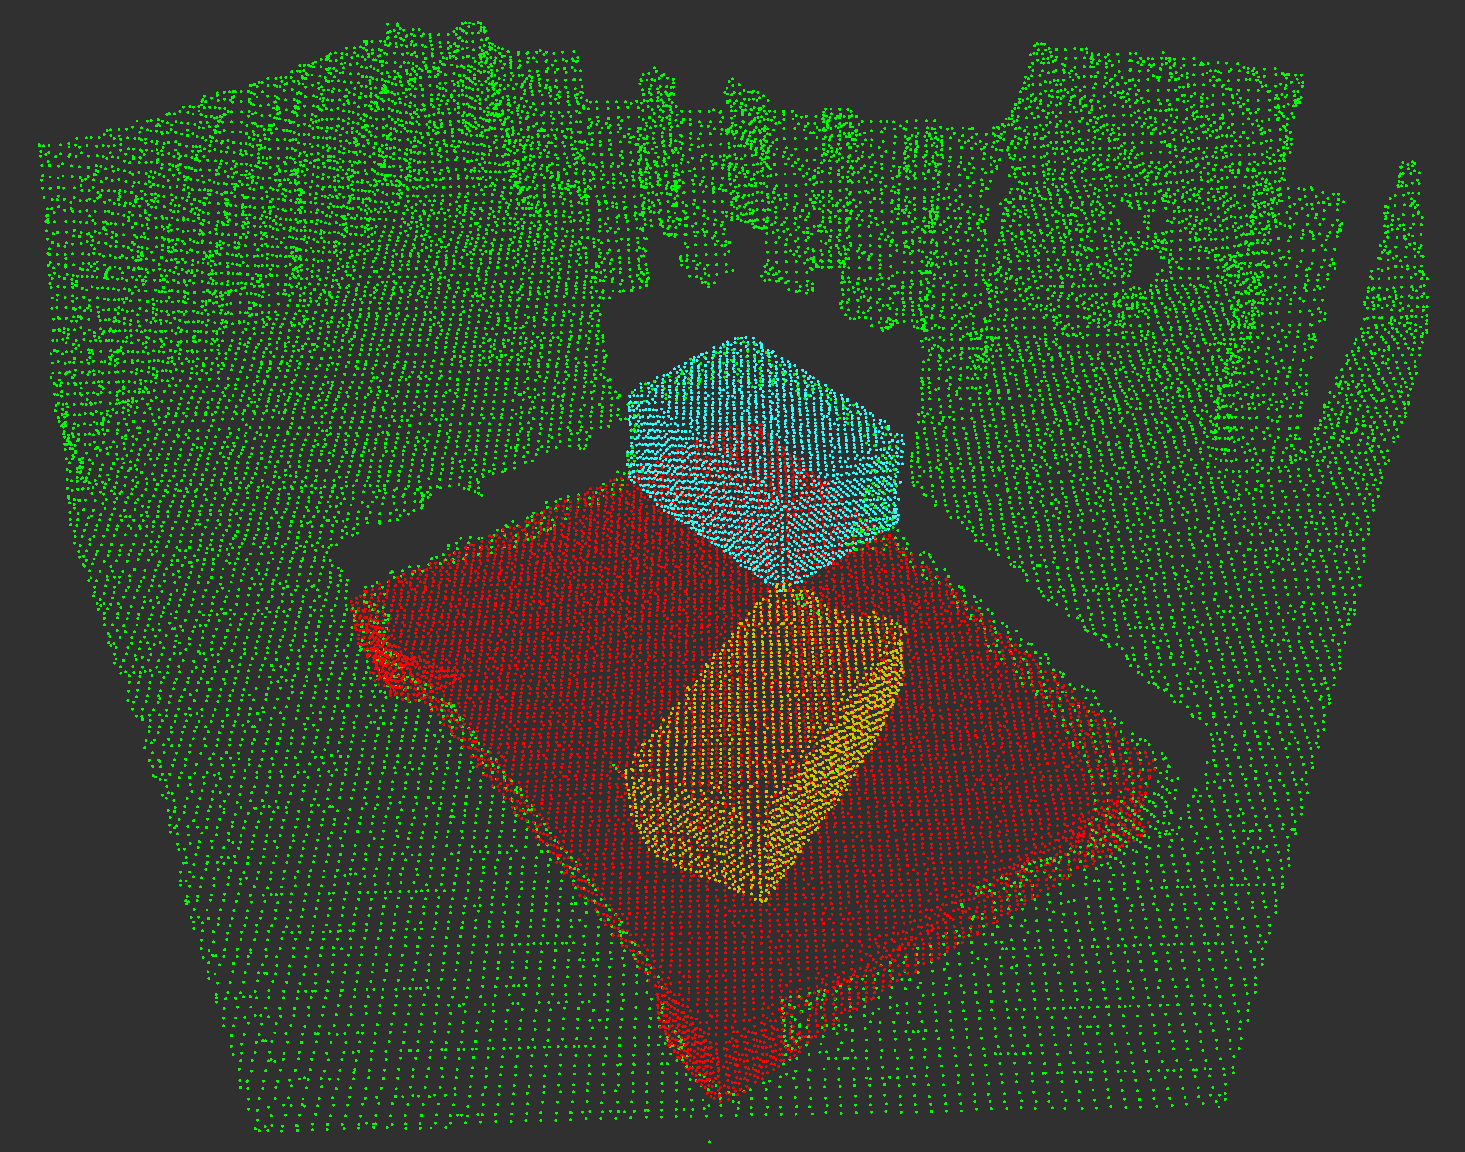
\includegraphics[width = 0.31\linewidth, height=3.0cm]{figs/collision_grid}
	    \label{fig:collision_grid}
}
\subfigure[] {
        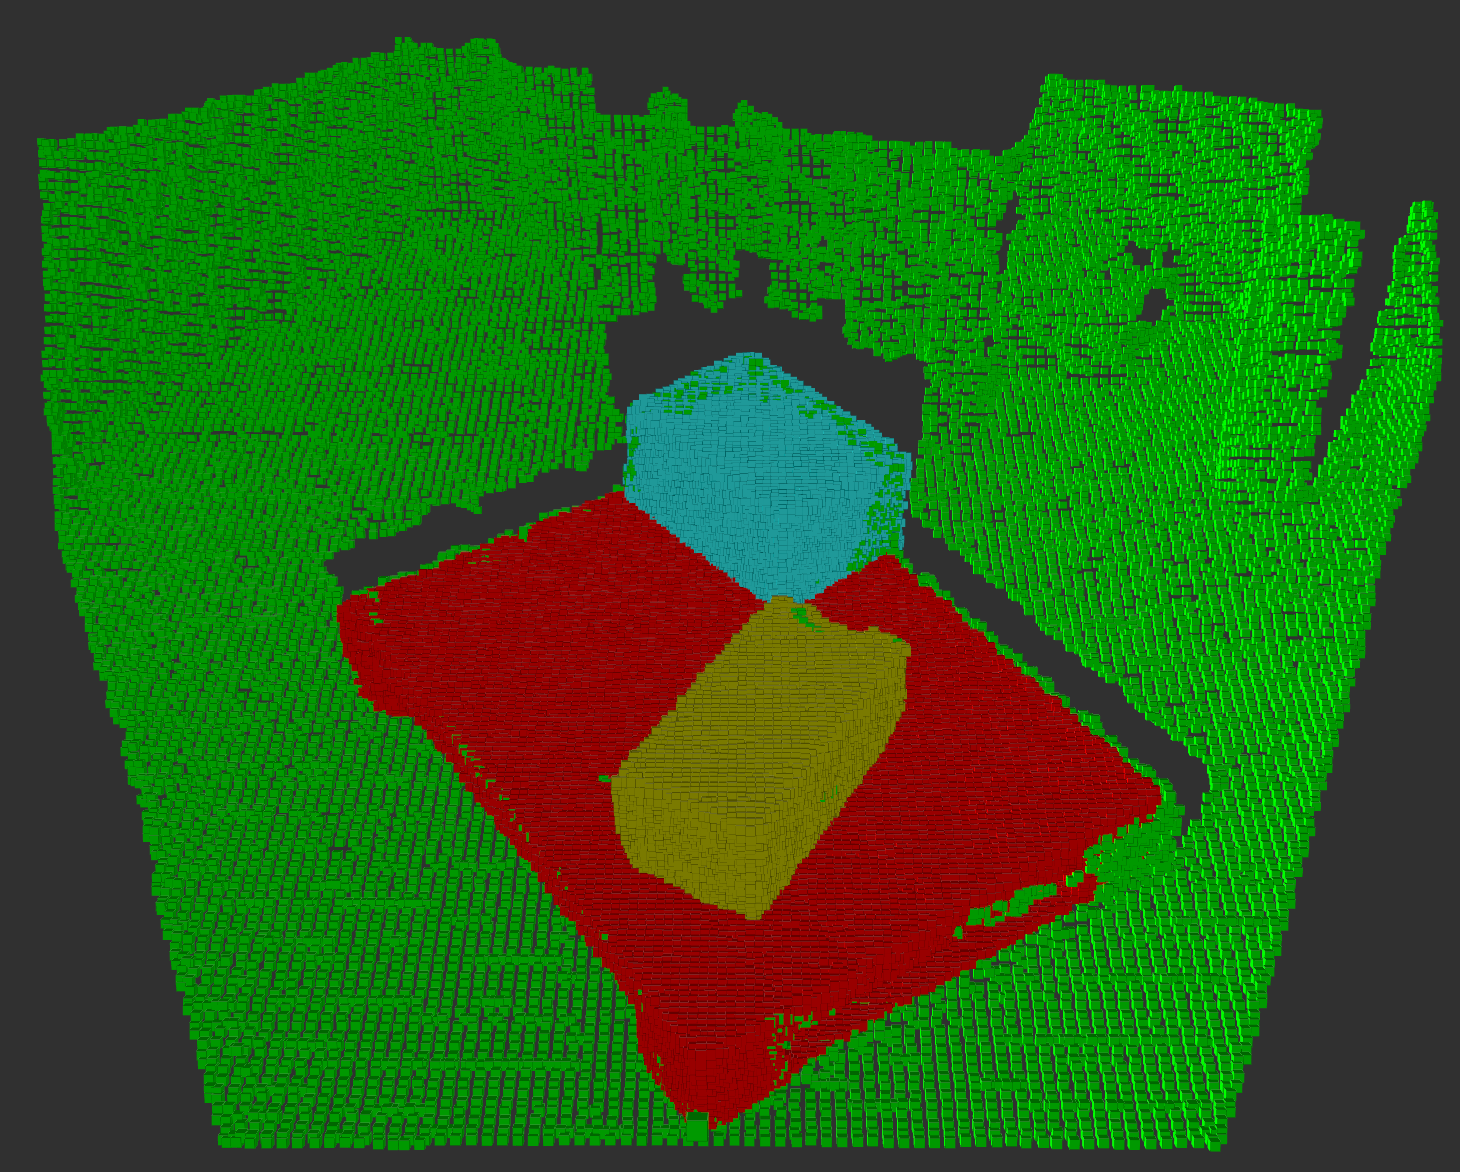
\includegraphics[width = 0.31\linewidth, height=3.0cm]{figs/valid_configs}
	    \label{fig:valid_configs}
}
\subfigure[] {
        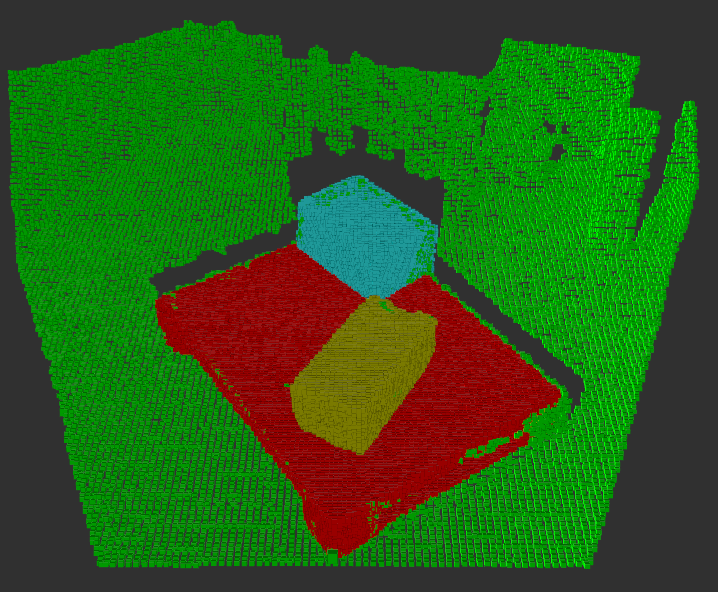
\includegraphics[width = 0.31\linewidth, height=3.0cm]{figs/distance_field}
	    \label{fig:distance_field}
}
\caption{Two-dimensional illustrations of the three main steps of our approach: \subref{fig:collision_grid} approach to pre-computing a collision map for the initial grasp envelope primitive; \subref{fig:valid_configs} three types of collisions which can occur and which are handled differently by our approach; \subref{fig:distance_field} process used for finding the maximum-volume cluster of valid grasp postures. The maximum-volume cluster in \subref{fig:distance_field} is shown in the shaded rectangle labeled \textbf{b}. }
\label{fig:method}
\end{figure*}
%
%

\begin{abstract}
Grasping systems that build upon meticulously planned hand postures rely on precise knowledge of
object geometry, mass and frictional properties --- assumptions which are often violated in
practice.
 In this work, we propose an alternative solution to the problem of grasp acquisition in simple autonomous pick and place scenarios, by utilizing the concept of grasp envelopes: sets of constraints on gripper postures.
We propose a fast method for extracting grasp envelopes for objects that fit within a known shape category, placed in an unknown environment.
Our approach is based on grasp envelope primitives, which encode knowledge of human grasping strategies.
We use environment models, reconstructed from noisy sensor observations, to refine the grasp envelope primitives and extract bounded envelopes of collision-free gripper postures.
Also, we evaluate the envelope extraction procedure both in a stand alone fashion, as well as an integrated component of an autonomous picking system.
\end{abstract}
%
\section{Introduction}
\label{sec:intro}
%
\begin{figure}[t!]
\centering
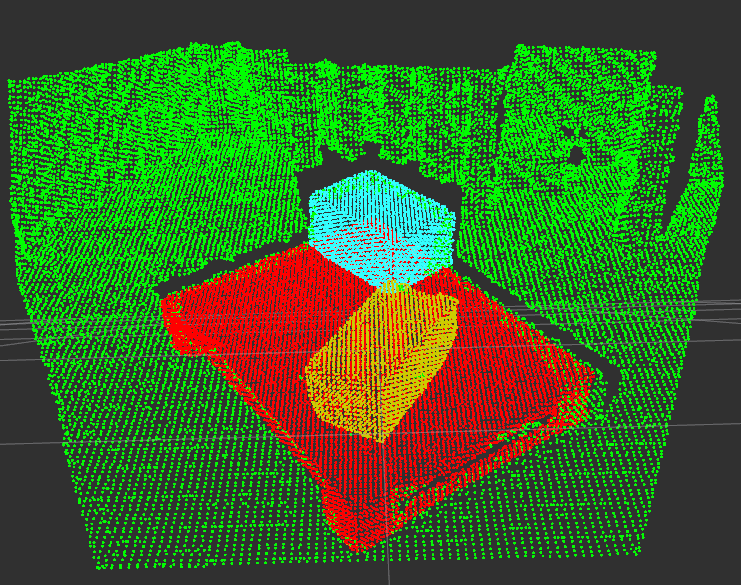
\includegraphics[width = \linewidth]{figs/setup}
\caption{The grasp envelope extraction procedure proposed in this work was used in an autonomous picking system, composed of the underactuated Velvet Fingers gripper~\cite{Tinc12} mounted on a KUKA LWR4+ robot arm (background). Experiments were performed to evaluate grasp acquisition success rates for the five test objects in the foreground. }
\label{fig:setup}
\end{figure}

Despite significant advances in gripper hardware design and in robot planning and control algorithms, autonomous grasp acquisition under uncontrolled conditions remains a challenging research problem.
On one hand, this is due to the necessity to solve a high-dimensional grasp- and motion planning problem for the full gripper-manipulator chain.
%
\par
%
The classical approach to reduce this complexity is to decouple the grasp synthesis problem by planning separately for the gripper and the manipulator.
To this end, state of the art grasping systems~\cite{Bere07,Srin10, Krug14a, Stoy15} often rely on sets of pre-computed grasps. 
At runtime, these grasps are evaluated by a motion planner and executed in an open-loop fashion, or in combination with perceptual feedback ($e.\,g.$, visual servoing).
 
%
\section{Related Work}
\label{sec:related}
As a comprehensive overview of data-driven grasp planning is beyond the scope of this work, we direct the interested reader to a recent survey by Bohg et al.~\cite{Bohg14} and only overview relevant approaches in constraint-based grasp representations.

In~\cite{Bere11}, TSRs are defined manually, while the main focus of our work is on extracting grasp envelopes in an automatic manner.
Our grasp envelopes can be seen as a generalization of TSRs with application to the grasping task, and can be readily integrated in the motion planning framework proposed by Berenson et al.
%
\par
The second set of approaches closely related to our work focus on the task of locating grasping affordances in various perceptual sensor data: for example, RGB images~\cite{Saxe08} or point clouds~\cite{Pas13}.
While there is a vast body of literature on extracting candidate grasps from various sensing modalities, most works concentrate on finding a single grasping configuration.
%
\section{Grasp Envelope Extraction}
\label{sec:method}
%%%%%%%%%%%%%%%%%%%%%%%%%%%%%%%%%%%%%%%%%%%%%%%%%%%%%%%%%%%%%%%%%%%%%%%%%%%%%%%%%%%%%%%%%%%%%%%%%%%%%%%%%%%%%%%%%%%%%%%
\begin{figure}[t!]
\centering
\subfigure[] {
        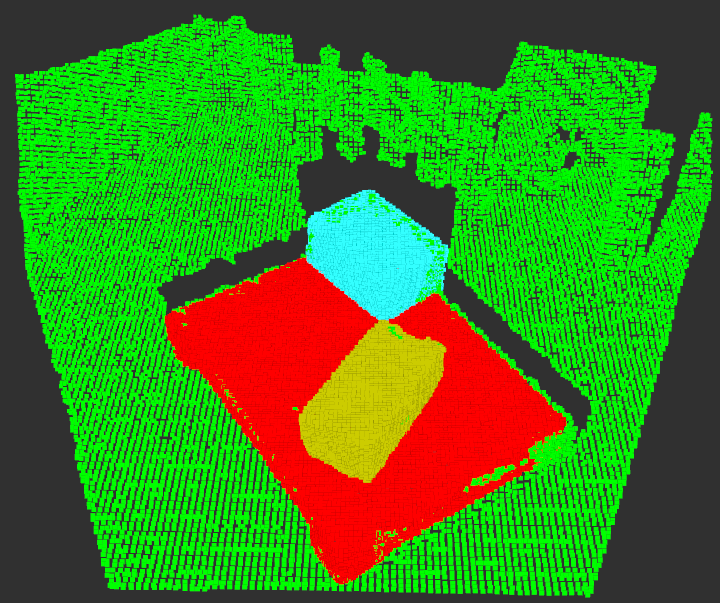
\includegraphics[width = 0.46\linewidth, height=3.5cm]{figs/primitive.png}
	\label{fig:grasp_primitive}
}
\subfigure[] {
        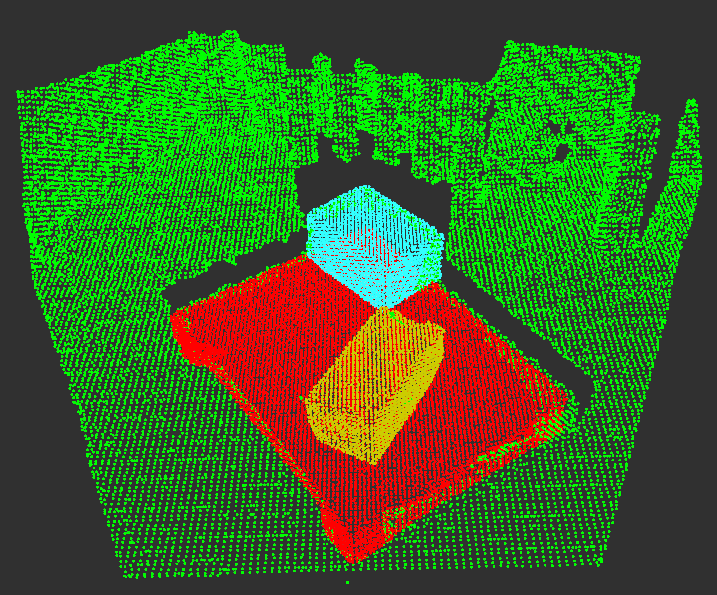
\includegraphics[width = 0.46\linewidth, height=3.5cm]{figs/truncated_raster_axis}
	\label{fig:grasp_interval}
}
\caption{An illustration of a cylindrical grasp envelope primitive in~\subref{fig:grasp_primitive}
  and a corresponding grasp envelope in~\subref{fig:grasp_interval}. The constraints are satisfied
  for any end effector pose which brings the gripper reference frame inside the shaded cylindrical
  shell sector, while maintaining orientation of the $x$ and $z$ axis within their respective shaded
  cone regions.}
\label{fig:grasp_envelope}
\end{figure}
%%%%%%%%%%%%%%%%%%%%%%%%%%%%%%%%%%%%%%%%%%%%%%%%%%%%%%%%%%%%%%%%%%%%%%%%%%%%%%%%%%%%%%%%%%%%%%%%%%%%%%%%%%%%%%%%%%%%%%%
\subsection{Grasp Envelopes}
Let $\mbm{p} = \left[x,y,z,o_x,o_y,o_z,o_w\right]^T$ be the pose of the gripper frame relative to a fixed frame connected to the robot kinematic model, represented by a 3D translation and a quaternion-encoded orientation. 
In addition, let $\mbm{q} \in \mathbb{R}^n$ be the configuration vector describing the joint angles of all $n$ gripper joints.
We represent the posture of the gripper as a vector $ \mbm{x} = \left[\mbm{p}^T, \mbm{q}^T\right]^T$.
We then define a grasp envelope $\mathcal{G}$ as a set of gripper postures satisfying constraints imposed on the gripper pose and joint configuration:
\begin{equation}
\mathcal{G} = \left\{ \mbm{x} \in \mathbb{R}^{n+7} \,|\, c_i(\mbm{x}) \leq 0,\, i = 1, \ldots, m \right\}
\label{eq:constraints}
\end{equation}
%
In this work, we restrict our analysis to linear inequality constraints, in order to facilitate an efficient implementation.
In addition, we concentrate our analysis on an underactuated gripping device with a single actuated degree of freedom, thus $q \in \mathbb{R}$. 
For simplicity, we only impose box constraints on the gripper opening angle, $i. \, e.$, $q_{min} \leq q \leq q_{max}$.
\par
The definition of a grasp envelope $\mathcal{G}$ in~\eqref{eq:constraints} allows us to encode various constraints on the robot end effector pose.
In this work we define two prototypical sets of grasp envelope constraints, which we term \textit{grasp envelope primitives} --- a cylindrical and a spherical primitive.
At runtime, the algorithms in Sec.~\ref{sec:collision_check} and~\ref{sec:fitting_bb} are used to refine the bounds on these primitives and obtain valid collision-free grasp envelopes for a particular object placement in the workspace.

An illustration of a cylindrical grasp envelope primitive is shown in Fig.~\ref{fig:grasp_primitive}, while a grasp envelope obtained by imposing additional bounds\footnote{In previous work~\cite{Krug15} we refer to this as a \textit{truncated} grasp envelope.} on the primitive is shown in Fig.~\ref{fig:grasp_interval}. 

Our treatment of the spherical shell grasp primitive is done in an analogous manner, by constraining
the gripper pose in between two concentric spheres while aligning the gripper's approach axis with
the vector pointing towards the sphere center and maintaining the gripper's lateral axis ($y$ in
Fig.~\ref{fig:grasp_envelope}) approximately parallel to a horizontal plane. 
\par
%%%%%%%%%%%%%%%%%%%%%%%%%%%%%%%%%%%%%%%%%%%%%%%%%%%%%%%%%%%%%%%%%%%%%%%%%%%%%%%%%%%%%%%%%%%%%%%%%%%%%%%%%%%%%%%%%%%%%%%
\begin{figure*}[t!]
\centering
\subfigure[] {
        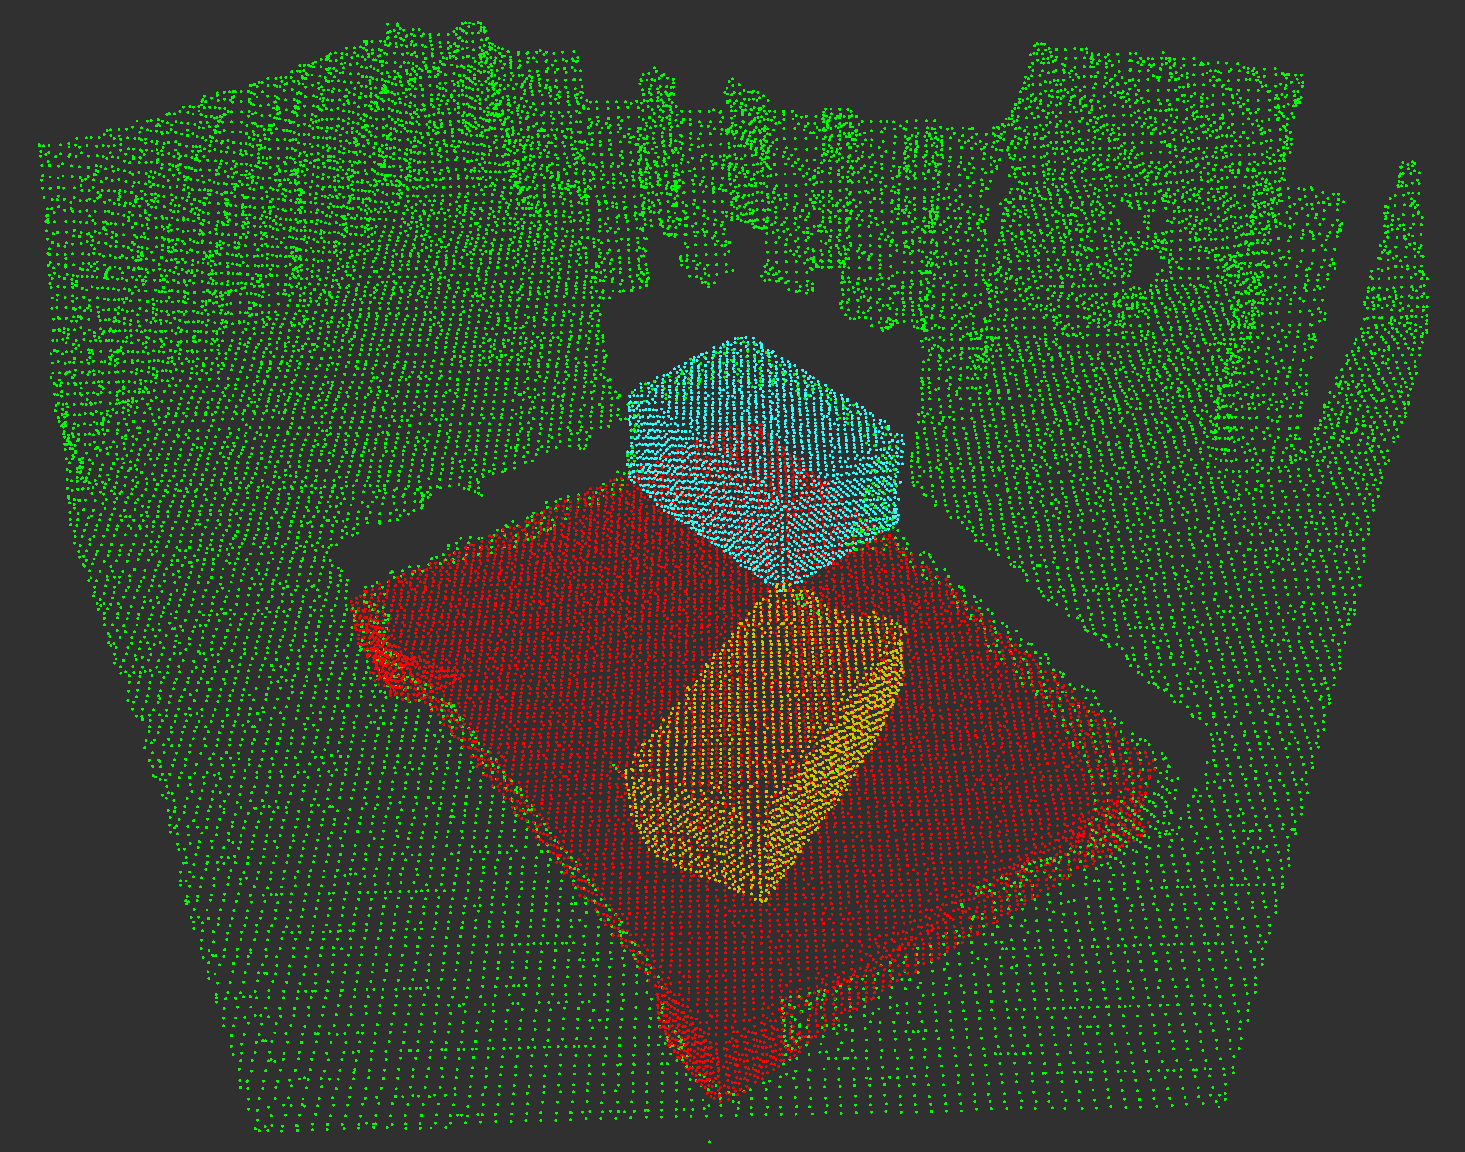
\includegraphics[width = .31\linewidth, height=5.0cm]{figs/collision_grid}
	    \label{fig:collision_grid}
}
\subfigure[] {
        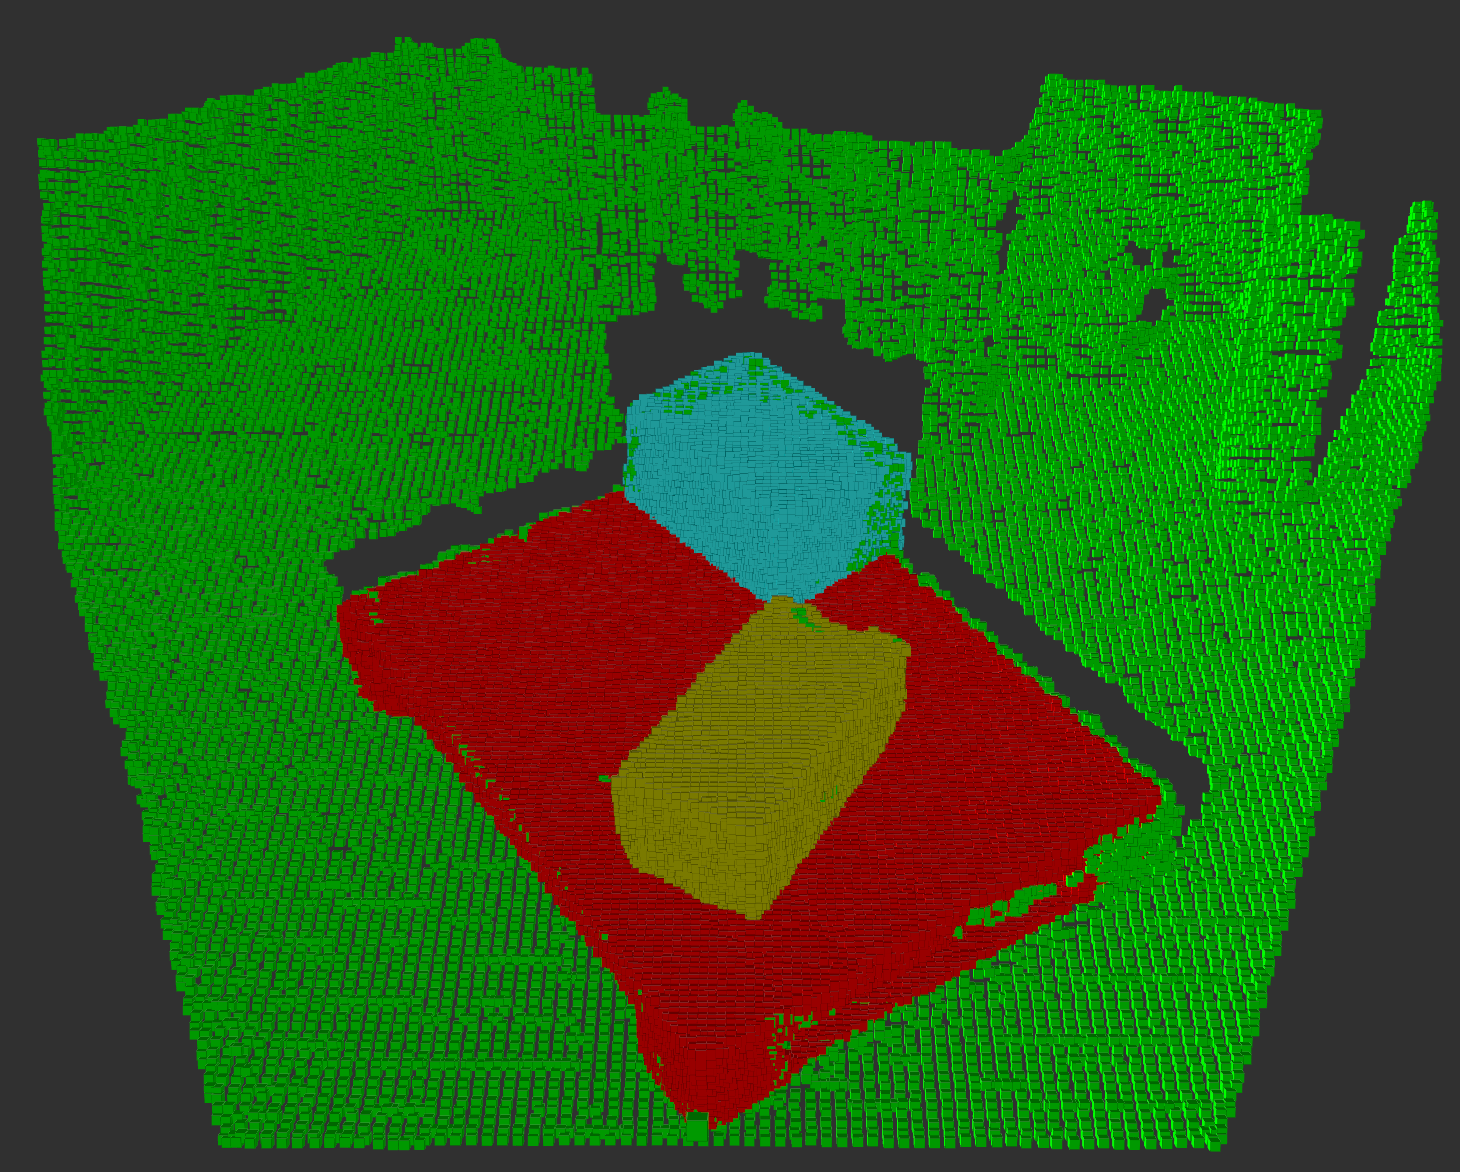
\includegraphics[width = .31\linewidth, height=5.0cm]{figs/valid_configs}
	    \label{fig:valid_configs}
}
\subfigure[] {
        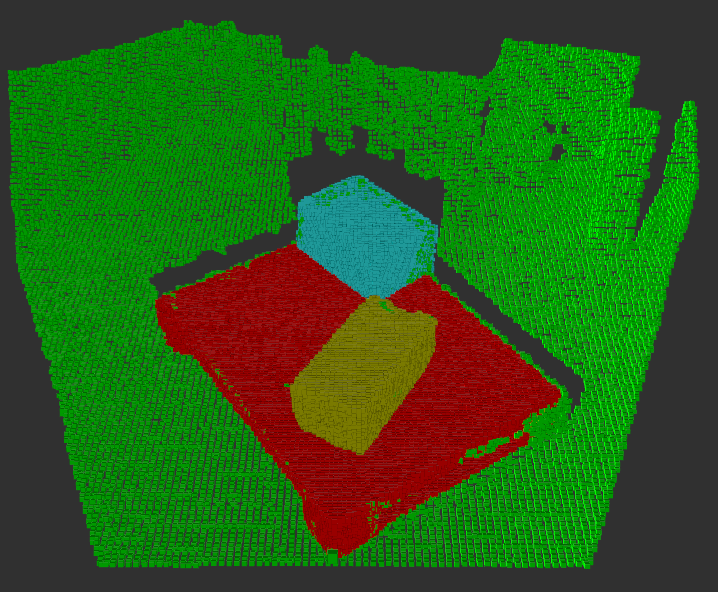
\includegraphics[width = .31\linewidth, height=5.0cm]{figs/distance_field}
	    \label{fig:distance_field}
}
\caption{Two-dimensional illustrations of the three main steps of our approach: \subref{fig:collision_grid} approach to pre-computing a collision map for the initial grasp envelope primitive; \subref{fig:valid_configs} three types of collisions which can occur and which are handled differently by our approach; \subref{fig:distance_field} process used for finding the maximum-volume cluster of valid grasp postures. The maximum-volume cluster in \subref{fig:distance_field} is shown in the shaded rectangle labeled \textbf{b}. }
\label{fig:method}
\end{figure*}
%%%%%%%%%%%%%%%%%%%%%%%%%%%%%%%%%%%%%%%%%%%%%%%%%%%%%%%%%%%%%%%%%%%%%%%%%%%%%%%%%%%%%%%%%%%%%%%%%%%%%%%%%%%%%%%%%%%%%%%
\subsection{Pre-computing a Collision Map}
\label{sec:sampling}
%
The first step of our approach is to pre-compute a 3D collision map for each of the two grasp envelope primitives.
This step is performed offline and greatly speeds up the subsequent online primitive refinement.
The procedure, illustrated by the 2D projection in Fig.~\ref{fig:collision_grid}, begins by sampling gripper poses from the initial envelope primitive.
We obtain the samples with a regular grid in the parametric space of each primitive and store them in a regular sample grid $\mathcal{S}$.
For the cylindrical shell primitive we sample along the distance to the center $d$, the orientation $\alpha$ (w.r.t. the cylinder  coordinate frame), and the height above the horizontal plane $h$. 
Similarly, the spherical shell primitive is parametrized by the radius $r$, and the polar and azimuth angles $\theta,\phi$.
\par
Next, for each sampled gripper pose we generate the gripper footprint in a collision map. 
As shown in Fig.~\ref{fig:collision_grid}, for this step we use an idealized gripper model, consisting of a bounding box around the palm and a semi-cylinder covering all possible placements of the fingers under different opening angles.
Each cell of the collision map covered by the ideal gripper footprint is then marked as occupied by the currently evaluated sample from $\mathcal{S}$. 
By iterating this procedure over all samples in $\mathcal{S}$ we obtain a collision map which encodes in every cell the list of gripper postures that would potentially occupy it.
%
%%%%%%%%%%%%%%%%%%%%%%%%%%%%%%%%%%%%%%%%%%%%%%%%%%%%%%%%%%%%%%%%%%%%%%%%%%%%%%%%%%%%%%%%%%%%%%%%%%%%%%%%%%%%%%%%%%%%%%%
\subsection{Finding Valid Configurations in Reconstructed Scenes}
\label{sec:collision_check}
Once we obtain the intersection between the two maps, we iterate through all affected cells in the collision map and check the affected gripper pose samples from $\mathcal{S}$.
As illustrated in Fig.~\ref{fig:valid_configs}, we distinguish between three types of collisions: 1) between the gripper palm and the map; 2) between the gripper fingers and the target object; and 3) between the fingers and other objects in the environment. 
Case 1) entails that the considered gripper pose would result in a collision, and thus we mark the corresponding sample in $\mathcal{S}$ as invalid.
Cases 2) and 3) would result in a collision only for specific configurations of the gripper opening angle $q$, thus we use them to impose tighter bounds on $q_{min}$ and $q_{max}$ associated with the respective sample in $\mathcal{S}$. 
At the end of this procedure we check the bounds on $q_{min},q_{max}$ for all remaining valid samples in $\mathcal{S}$ and invalidate those that impose infeasible constraints ($i.\,e.$, $q_{min}\geq q_{max}$) and those that would not result in a grasp of the target object ($q_{min} = 0$ when no contact with the object was detected).

\subsection{Fitting a Maximum Volume Envelope}
\label{sec:fitting_bb}
%
Following the procedures outlined in the previous subsections, we obtain a grid of discrete samples $\mathcal{S}$ representing a set of gripper postures.
Some of the postures in $\mathcal{S}$ have been invalidated by the collision checks in Sec.~\ref{sec:collision_check}, while the remaining ones are valid under certain bounds on $q$.
In order to obtain a refined grasp envelope following the definition in \eqref{eq:constraints}, we need to find a set of inequality constraints in Cartesian space containing only valid samples from $\mathcal{S}$. 
Thanks to our regular grid sampling strategy from Sec.~\ref{sec:sampling}, it is straightforward to obtain a set of Cartesian-space constraints for any axis-aligned bounding box in $\mathcal{S}$.
Thus, we can obtain a refined grasp envelope by looking for the largest axis-aligned inscribed box in $\mathcal{S}$: $i.\,e.$, the maximum volume box containing only valid samples.
\par
Finding maximum volume/area inscribed shapes is in general a hard problem.
Our problem instance is however additionally constrained to a regular sample grid and axis aligned shapes, and can therefore be solved efficiently.
If we treat invalid samples in $\mathcal{S}$ as occupied space, and conversely valid samples as free space, we can use a variant of the distance transform to speed up our search.
In general, we are looking for a $k$ dimensional axis-aligned bounding box, with $k$ being the dimensionality of the sampling grid $\mathcal{S}$. 
For simplicity, in this section we discuss a 2D version of our approach (illustrated in Fig.~\ref{fig:distance_field}), which is readily extendable to $k$D.
The main idea here is to look for the best position of the lower-right corner of the maximum bounding rectangle (the shaded rectangle labeled \textbf{b} in Fig.~\ref{fig:distance_field}).
We first construct a 2D distance field which for every free cell encodes the distance to the closest occupied cell in the negative direction ($i.\,e.$, towards the upper-left corner), along each dimension.
This provides us with an absolute upper bound on the volume of a box which uses a particular cell as a lower-right corner: $e.\,g.$, the example labeled \textbf{a} in Fig.~\ref{fig:distance_field} would result in a maximal volume of $8\times5=40$ samples.
Using this as a criterion to prune the search space, Algorithm~\ref{alg:bbsearch} can be used to find the maximal-area box. 
Lines 8-15 in the algorithm describe the search procedure along the $x$ direction of the distance grid, as shown also in case \textbf{b} of Fig.~\ref{fig:distance_field}.
In essence, we keep track of the maximum area rectangle verified so far ($m_i,m_j$), and update it for every slice along $x$ in lines 10-11. 
We next check if it is possible to obtain a larger area rectangle (in the best case) if we continue searching.
If so, we refine the boundary $d_j$ along $y$ (lines 12-13), otherwise we stop the search (line 15).
Last, we check if the rectangle obtained in this manner is larger than the current best candidate and move to the next possible bottom-right corner (lines 18-19).
For the envelope primitives discussed in this work, $k=3$ and we obtain a straight-forward extension of the presented algorithm to 3D by searching in addition along the third dimension.
At a moderate computational cost, this algorithm can be modified to extract the top $N$ largest volume regions. 
Finally, since the zero position for sampling dimensions associated with varying orientation is arbitrary, in these cases we allow regions to span across the first-to-last element border and modify the distance field computation accordingly.
\begin{algorithm}[t!]
\DontPrintSemicolon % Some LaTeX compilers require you to use \dontprintsemicolon instead 
\KwIn{Distance transform $D$}
$V_{max} \gets 0$\;
%\For{$x,y \gets 1$ \textbf{to} $|D|_x,|D|_y$}{
\For{$\forall$ cells in $D$}{
    Let $i,j \gets$ index of current cell, $D_{i,j}^x,D_{i,j}^y\gets$ value of $D$ at $i,j$ along $x,y$ dimensions \;
    \If{$(i-D_i)(j-D_j) > V_{max}$} {
	$m_i,m_j \gets 0$ \;
	$d_i,d_j \gets D_{i,j}^x,D_{i,j}^y$ \;    
	//search along $x$ \;
	\For{$k\gets i$ \textbf{to} $i-D_i$} {
	    $d_{min} \gets min(d_j,D_{k,j}^y)$ \;
	    \If{$(k-i) d_{min}> m_i m_j$ } {
		$m_i,m_j \gets k-i, d_{min}$ \;
	    }
	    \If{ $d_i d_{min} > m_i m_j$} {
		$d_j \gets d_{min}$ \;
	    }	
	    \Else {
		break \;
	    }
	}
	//search along $y$ equivalent \;
	$\ldots$ \;
	\If{$(i-m_i)(j-m_j) > V_{max}$} {
	    $V_{max} \gets (i-m_i)(j-m_j)$, store bounds \;
	}
    }
}
\Return{$V_{max}$, bounds}\;
\caption{{\sc BBSearch2D:} find largest rectangle}
\label{alg:bbsearch}
\end{algorithm}

%
\section{Evaluation}
\label{sec:results}
\subsection{Envelope extraction evaluation}
\label{sec:offline_tests}
%
\begin{figure*}[t!]
\centering
\subfigure[] {
        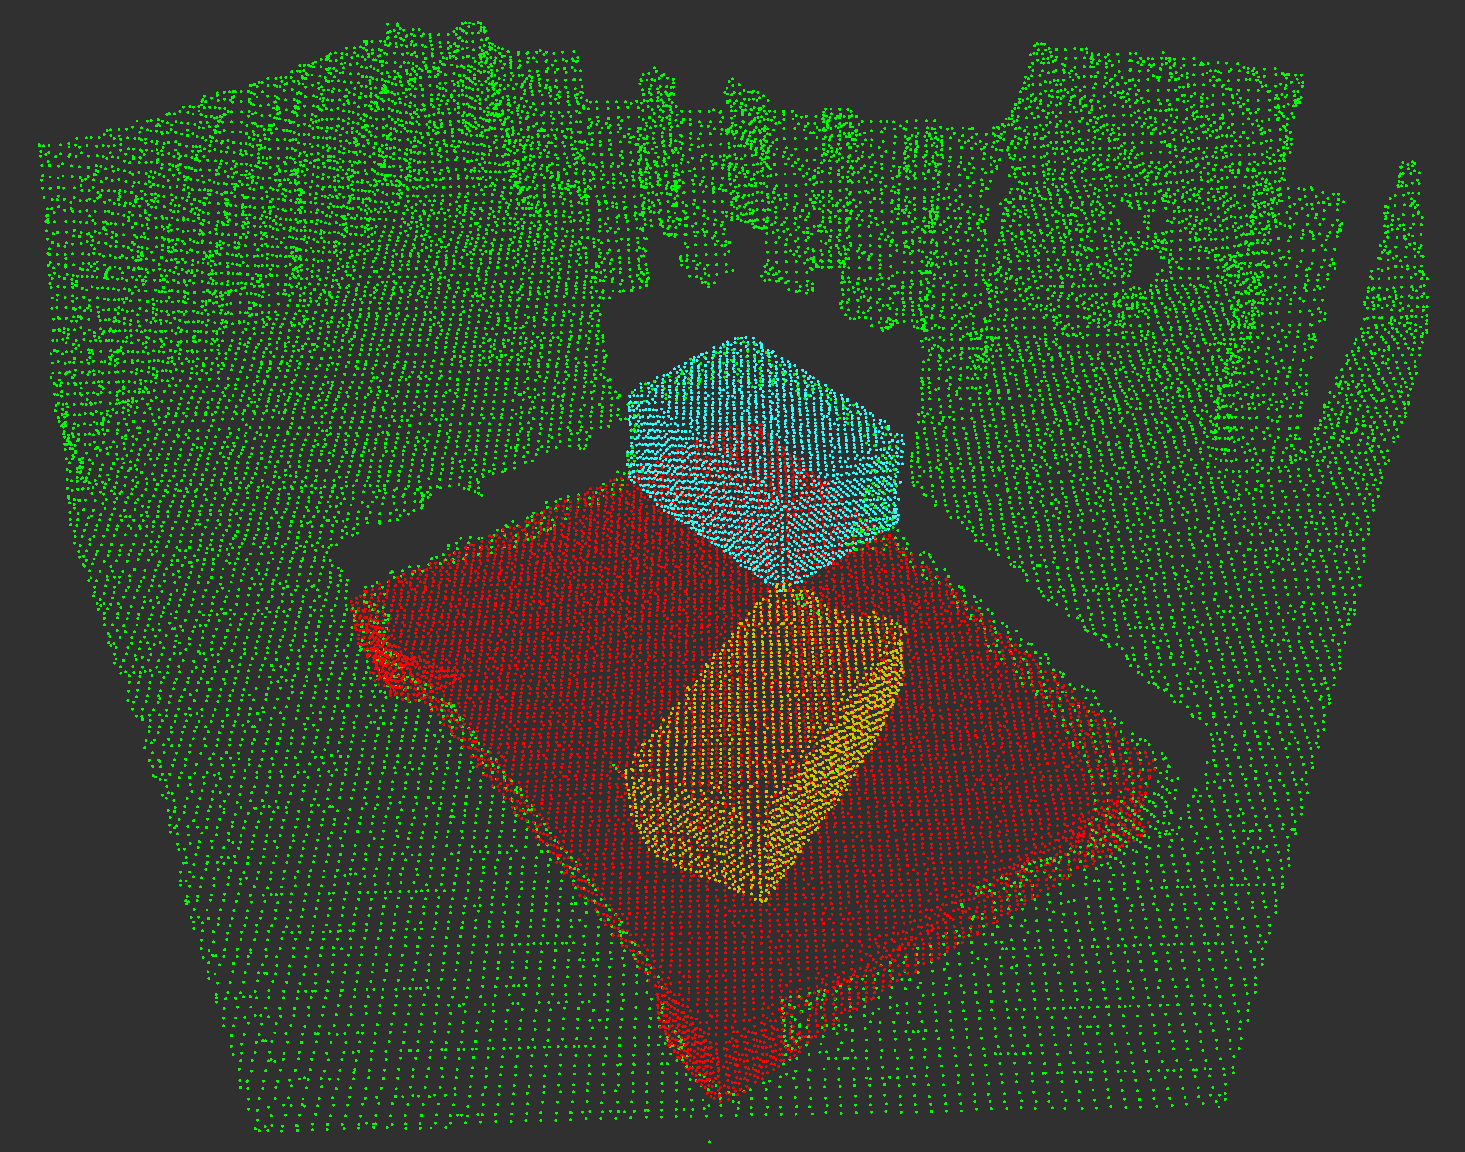
\includegraphics[width = 0.46\linewidth, height=6.0cm]{figs/shelves}
	\label{fig:shelves}
}
\subfigure[] {
        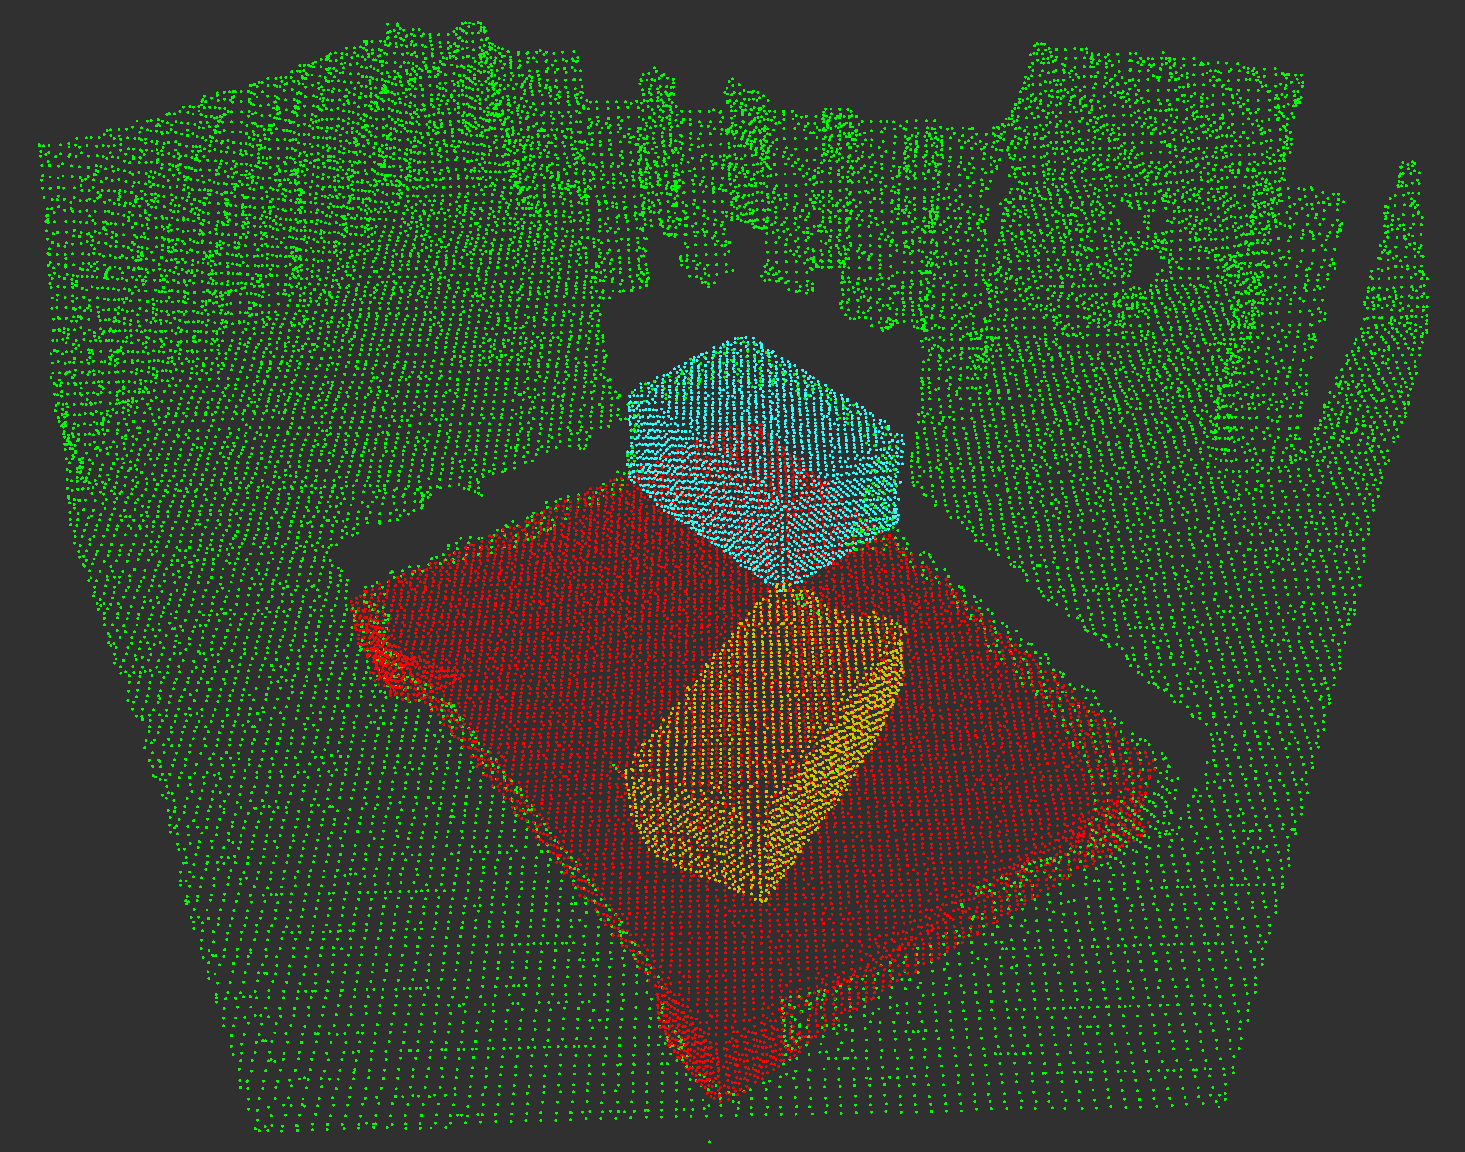
\includegraphics[width = 0.46\linewidth, height=6.0cm]{figs/tables}
	\label{fig:tables}
}
\caption{Illustration of the test environments used in this paper: \subref{fig:shelves} shows the TSDF models of the five scenes from the \textit{shelves} data set, reconstructed at $5$~mm resolution; \subref{fig:tables} shows the models of the \textit{table} data set at $10$~mm resolution.}
\label{fig:environments}
\end{figure*}
%
%\begin{figure}[t!]
%\centering
%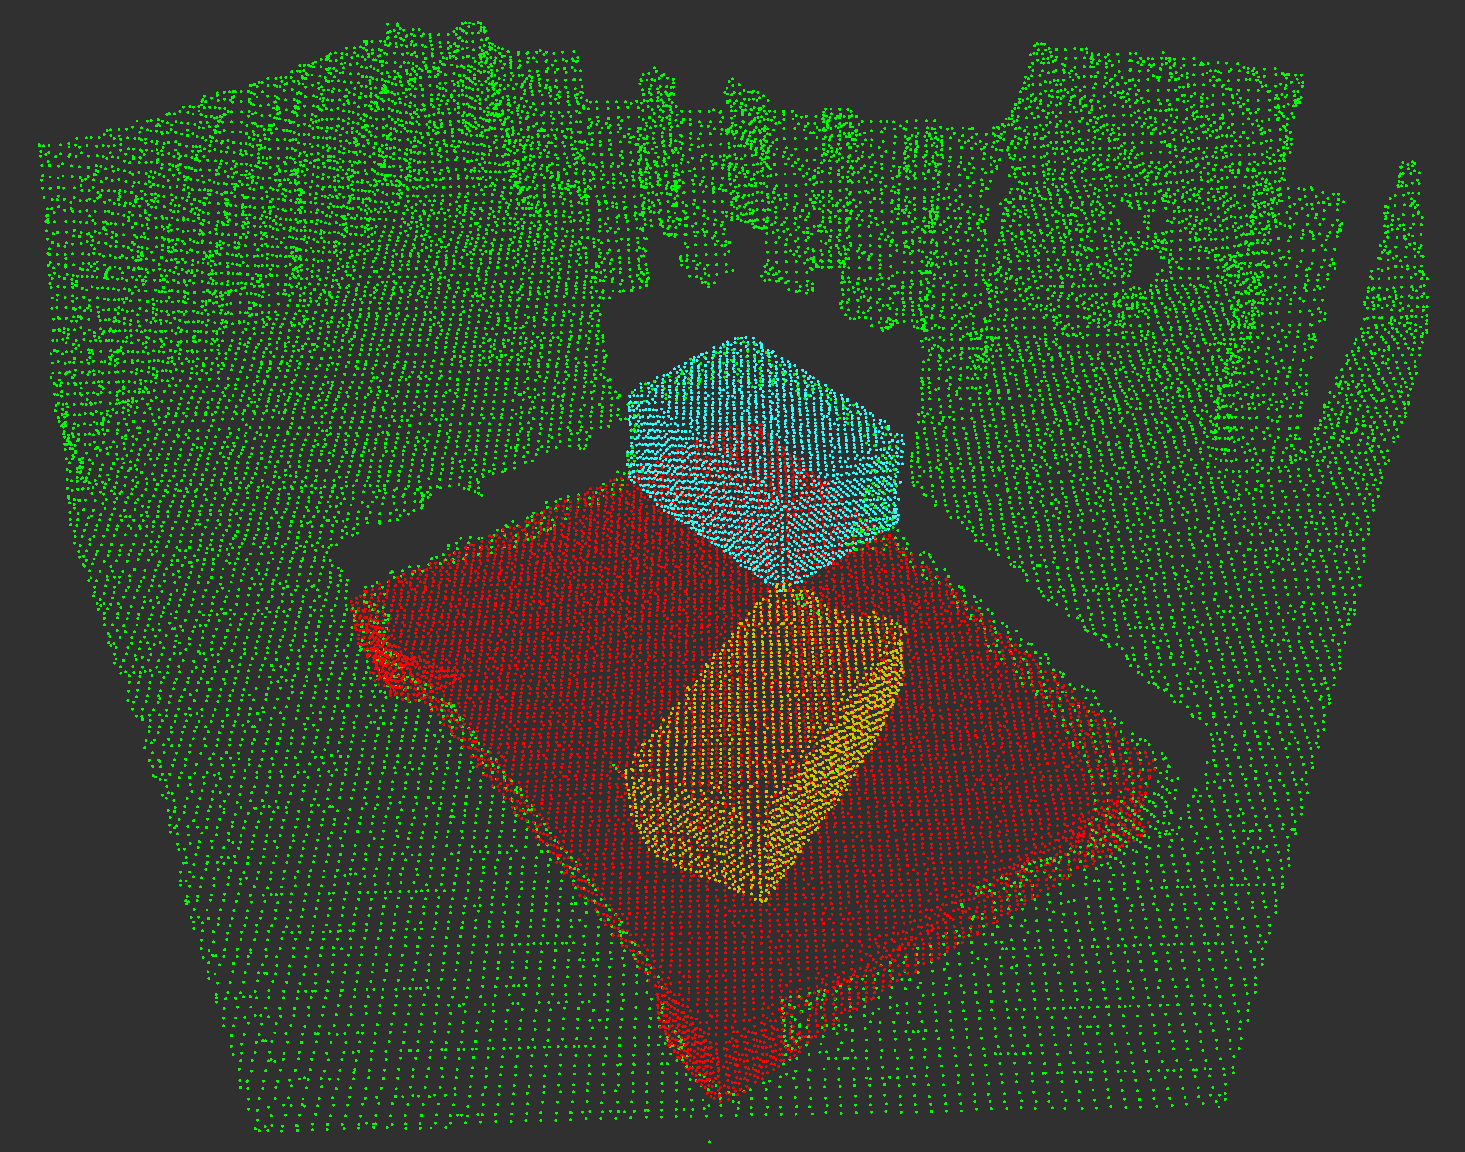
\includegraphics[width = .9\linewidth]{figs/objects}
%\caption{The five test objects used in the evaluation. The two plush toys were evaluated with spherical envelope primitives fit to the head, while the remaining objects were associated with cylindrical primitives.}
%Cup\label{fig:objects}
%\end{figure}
As a first step, we evaluated the proposed grasp envelope fitting approach on a set of five test
objects placed in ten different scenes. Here, the purpose was to evaluate the computational effort
of the envelope extraction procedure, as well as the quality of the obtained envelopes. Under the assumption
that all grasps which respect the envelope constraints are successful, envelope quality $Q$ is
defined as the number of valid gripper pose samples from $S$ that fall within the grasp envelope. This measure
directly relates to the enclosed volume of the envelope constraints. Thus, envelopes with larger
quality $Q$ allow for more gripper pre-grasp posture redundancy and easier grasp acquisition. Two plush toys (a teddy bear and a pig), a water bottle, a large cup and a cardboard box (shown in
Fig.~\ref{fig:objects}), all graspable by the considered gripping device, were chosen as target objects.
We placed the objects in different poses in two different types of scenes, models of which are shown in Fig.~\ref{fig:environments}. 
For the first set of five scenes, the objects were placed on shelves in an office environment, resulting in a moderately cluttered setup.
Conversely, in the second set, objects were placed on a table top and were spaced further apart from each other.
These two sets of environments (referred to as the \textit{shelves} and \textit{table} data sets) were scanned using a hand-held Asus Xtion Pro\footnote{\url{http://www.asus.com/Multimedia/Xtion_PRO_LIVE/}} RGB-D camera.
The sensor pose was tracked using the SDF Tracker algorithm~\cite{Cane13a}.
The shelves data set was reconstructed at grid resolutions of $5$~mm and $10$~mm, while the table data set was reconstructed only at a resolution of $10$~mm, as the lower number of geometrical features in the latter caused bad tracker performance at higher grid resolutions.
Object poses and bounding sphere/cylinder size were manually determined for each test case.
\par
We pre-computed two sets of spherical and cylindrical grasp envelopes, using collision grid resolutions of $5$~mm and $10$~mm respectively.
For the cylindrical envelopes, we sampled poses at $15$ radial distances with $0.1$~m $\leq d \leq 0.3$~m, $100$ orientations with $0\leq \alpha \leq 2\pi$~rad and $7$ vertical slices over a span of $0.2$~m.
The spherical primitive was sampled at $15$ distances $r$ and $100$ orientations, using the same metric bounds, as well as $7$ different inclinations.
In both cases, this resulted in a 3D sampling grid $\mathcal{S}$ of $10500$ gripper poses.
A visual example of the results obtained for the extracted grasp envelope of one of the objects in the shelves data set is shown in Fig.~\ref{fig:example}.
%\begin{figure}[t!]
%\centering
%\includegraphics[width = \linewidth]{figs/grasp_illustration_v2}
%\caption{Illustration of the test environments used in this paper: \subref{fig:example}}
%\label{fig:example}
%\end{figure}
\par
In addition to visual inspection, we also measured for each grasp envelope the computation time
spent in extracting it and the quality metric $Q$. Fig.~\ref{fig:result} shows a boxplot of the
obtained envelope qualities per object and data set, with each box centered on the mean and spanning
the area between the $25$th and $75$th percentile. We can draw several conclusions from the results
shown in Fig.~\ref{fig:result}. First, it is evident that the less cluttered table data set results
in substantially larger grasp envelopes, validating that the proposed method is able to find grasp
envelopes with higher quality for objects that are easier to grasp.
Second, by comparing results on the two reconstructions of the shelves data set, we note that the grasp envelopes extracted from higher resolution models are slightly larger.
This effect is due to the more precise collision checks performed.
However, in our tests the performance gain by using a higher resolution does not seem significant, most likely owing to the fact that the amount of clutter in the scenes is not extremely high.
As this performance gain comes at a price of an order of magnitude slower computational time, we conclude that very precise environment models should only be utilized when necessary.
Finally, we note that the performance of the proposed method is worst for the cup object. 
Upon further investigation, this artifact can be explained by a particularity of the TSDF representation used to model the environment: it is particularly susceptible to modeling errors on thin objects observed from multiple viewpoints. 
As both the outer and inner walls of the cup are often visible in our data sets, the fidelity of the models is often not optimal, resulting in lower certainty on the extracted grasp envelopes.
Regarding computational performance, our approach extracts grasp envelopes in roughly $200$~ms at a resolution of $5$~mm and  $20-40$~ms at a $10$~mm resolution (using a single core of an Intel Xeon CPU E5-1620 v3 at 3.50GHz).
Most of the time is spent on computing the valid samples as per Sec.~\ref{sec:collision_check}, with only a small fraction of resources expended on extracting the maximum volume envelope.
%
\begin{figure*}[t!]
\centering
\subfigure[] {
        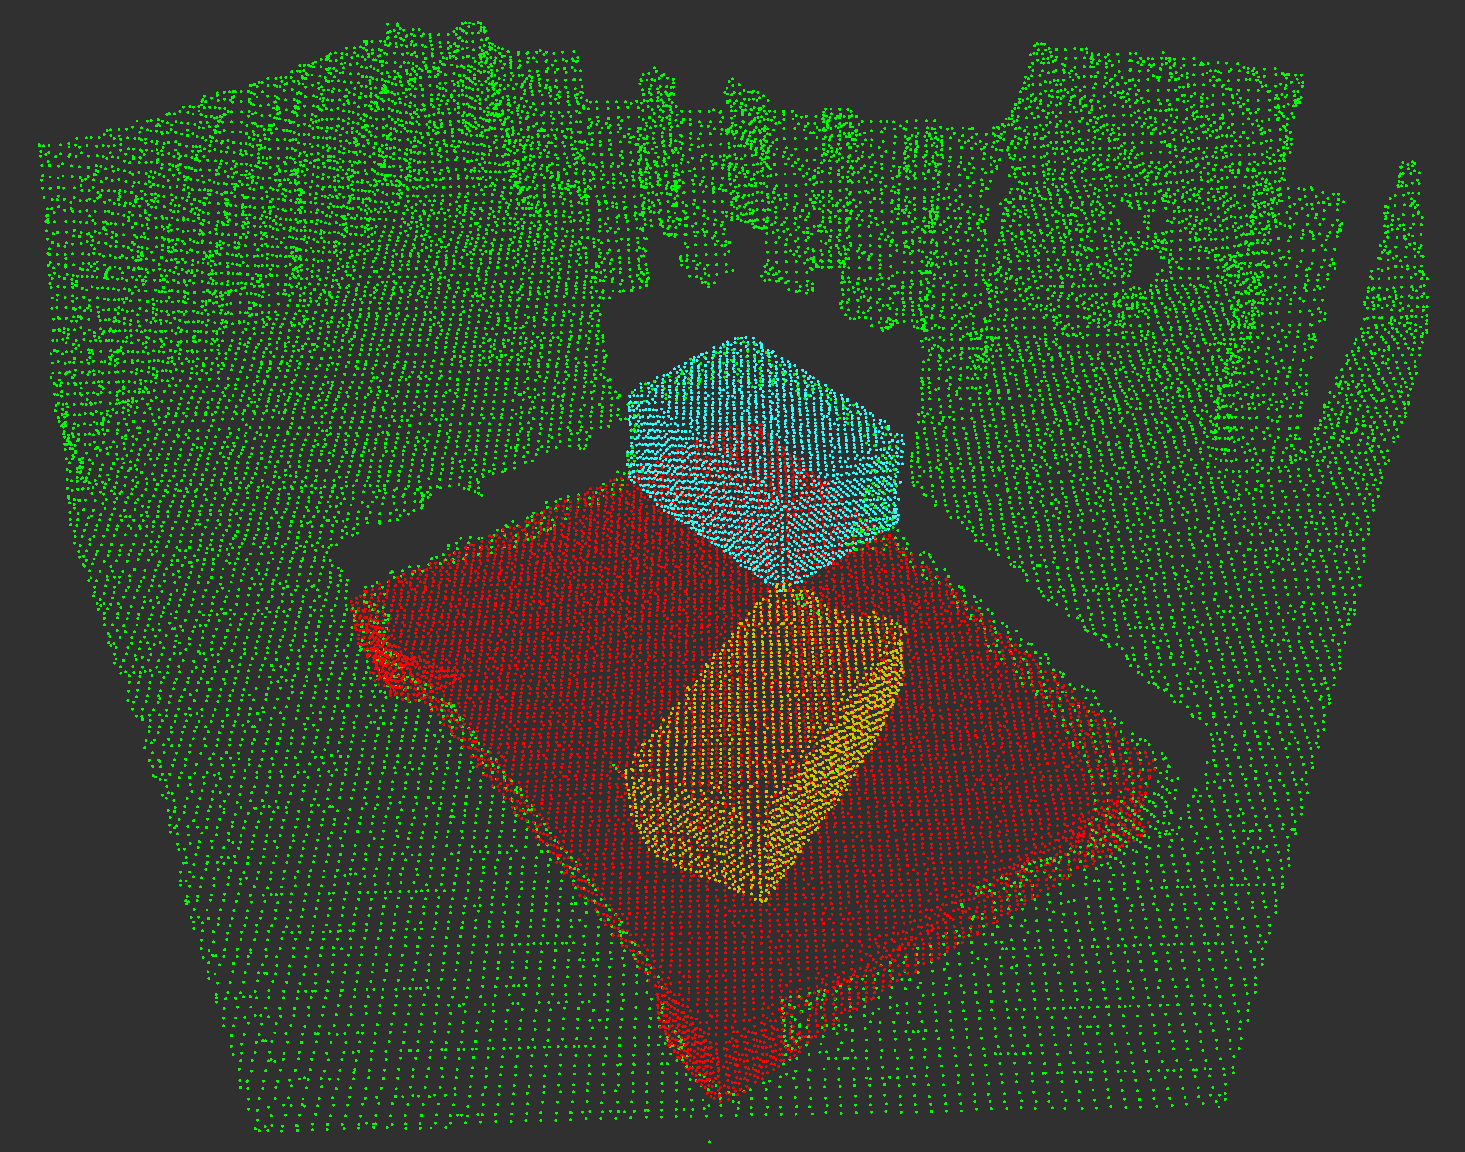
\includegraphics[width = 0.3\linewidth, height=5.0cm]{figs/objects}
	\label{fig:objects}
}
\subfigure[] {
        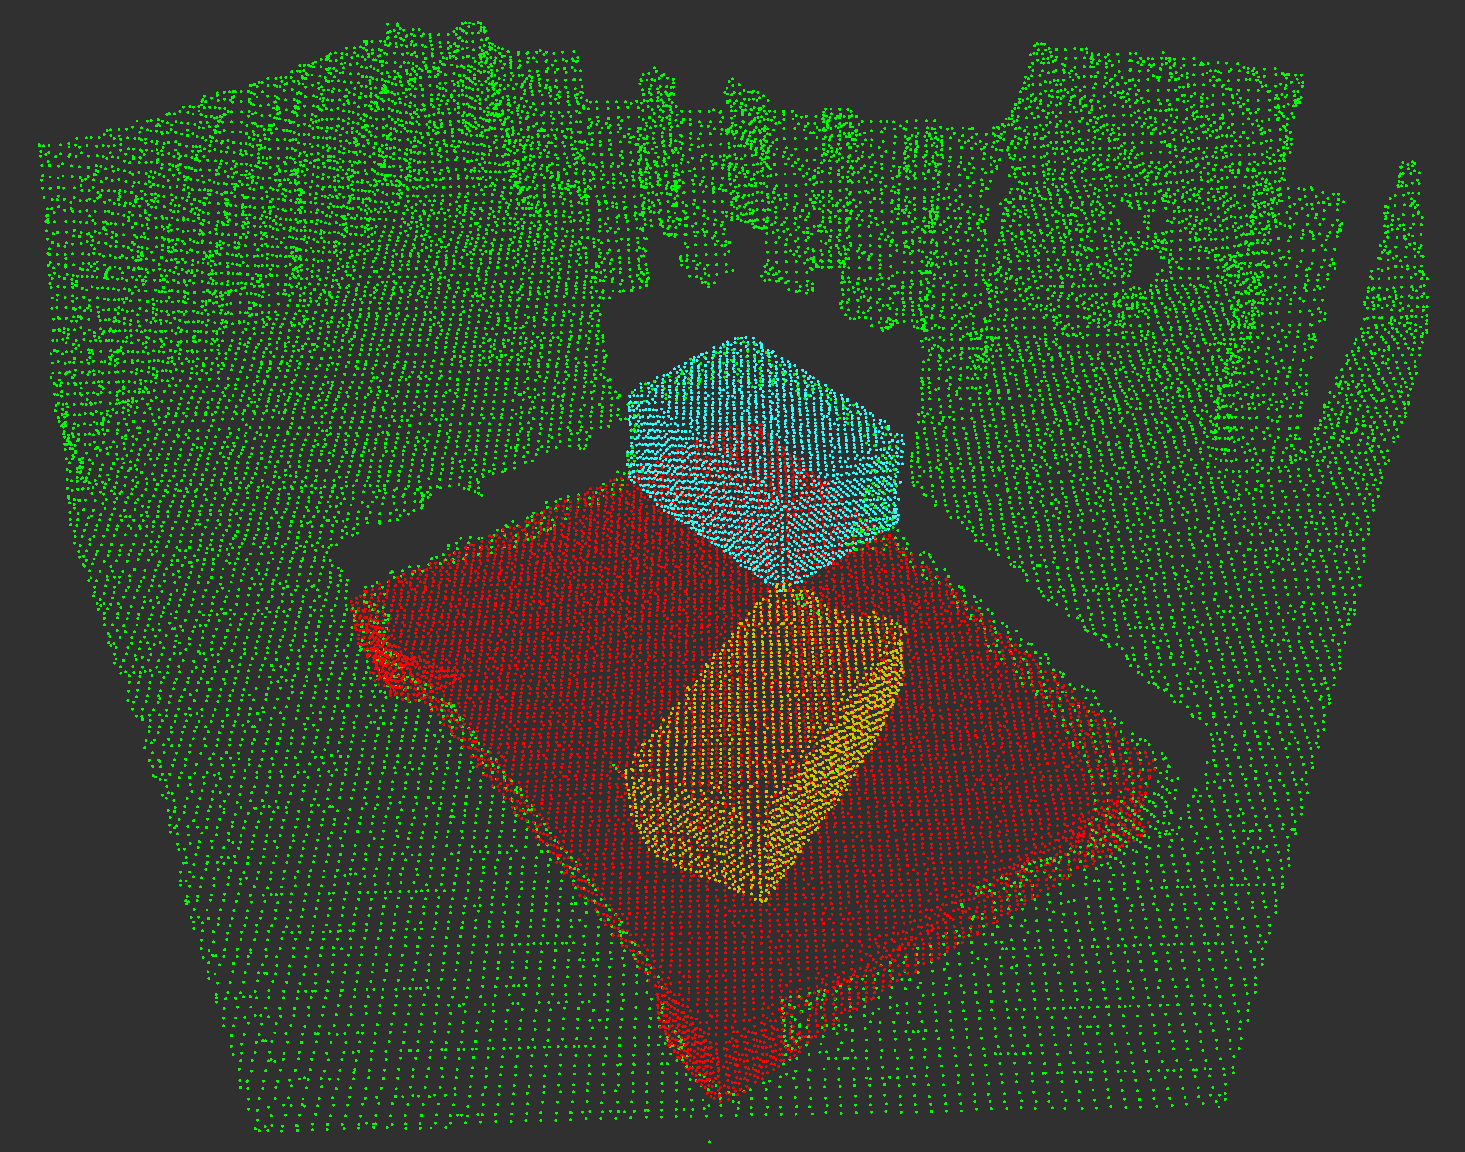
\includegraphics[width = 0.3\linewidth, height=5.0cm]{figs/grasp_illustration_raster}
	\label{fig:example}
}
\subfigure[] {
        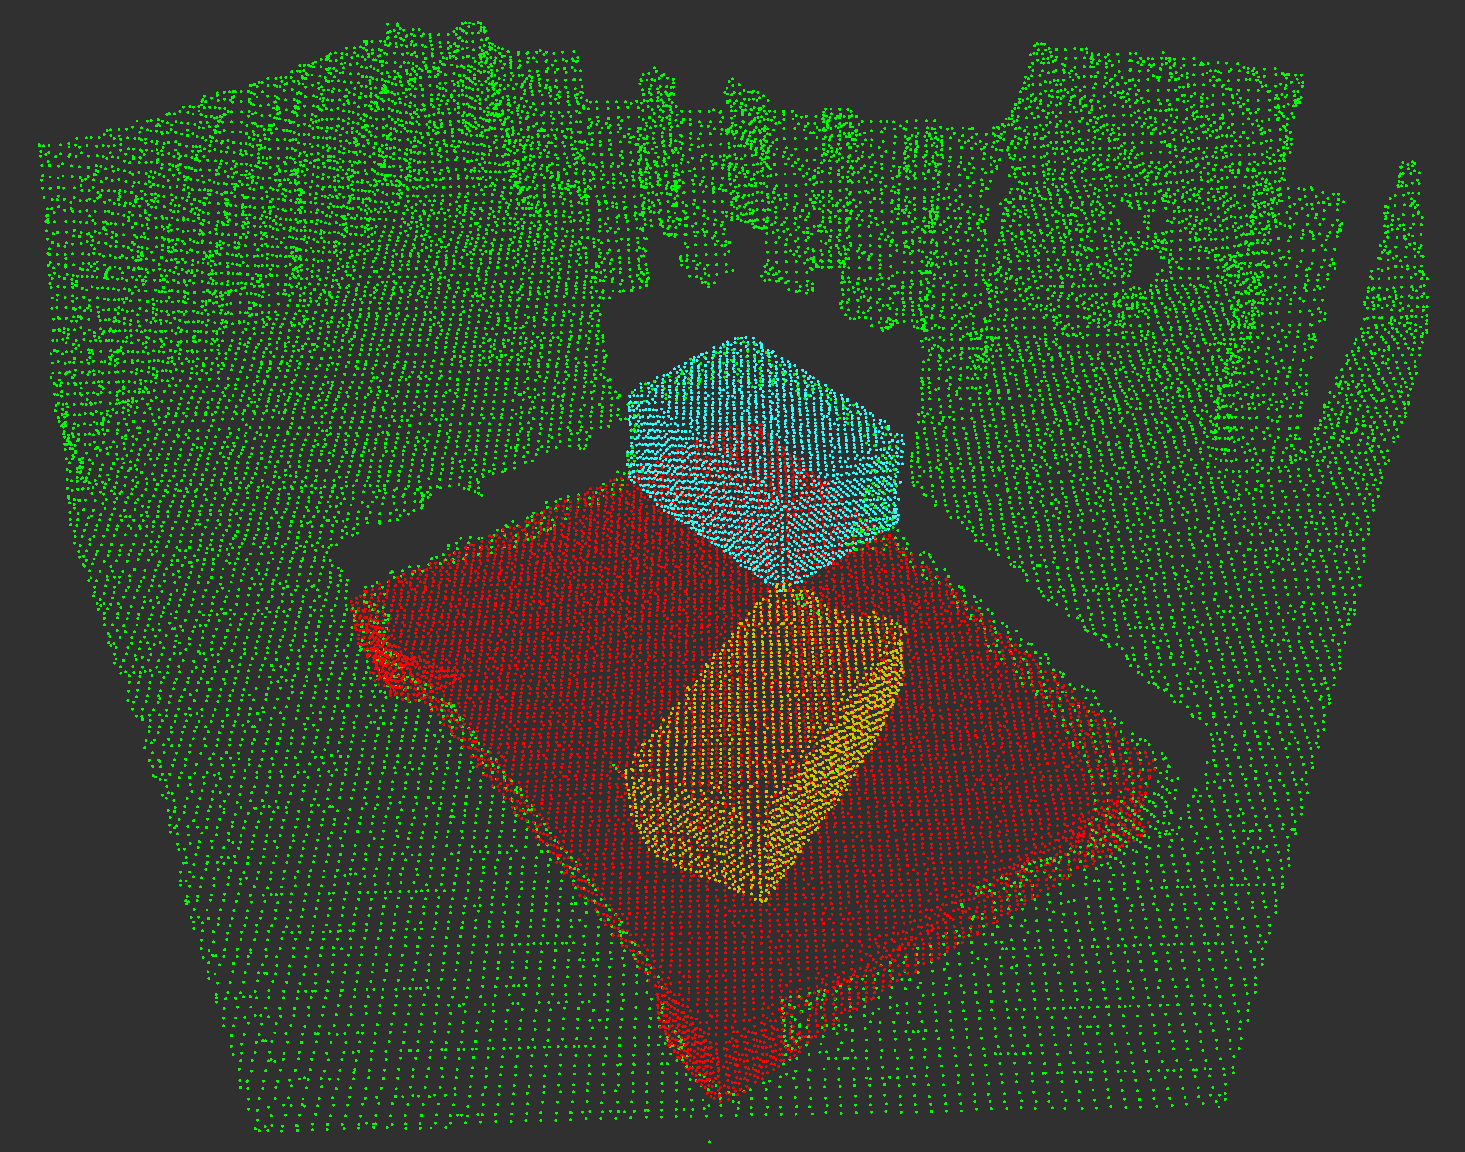
\includegraphics[width = 0.3\linewidth, height=5.0cm]{figs/results}
	\label{fig:result}
}
\caption{\subref{fig:objects} shows the five test objects used in the evaluation. The two plush toys were evaluated with spherical envelope primitives fit to the head, while the remaining objects were associated with cylindrical primitives. \subref{fig:example} illustrates typical constraint envelopes extracted for objects in cluttered environments; \subref{fig:result} summarizes results of the proposed grasp envelope extraction method, showing the distribution of envelope quality $Q$ over different objects and scenes. }
\label{fig:results}
\end{figure*}
%
\subsection{Grasp acquisition success evaluation}
\label{sec:online_evaluation}
%
\begin{figure*}[t!]
\centering
\subfigure[] {
        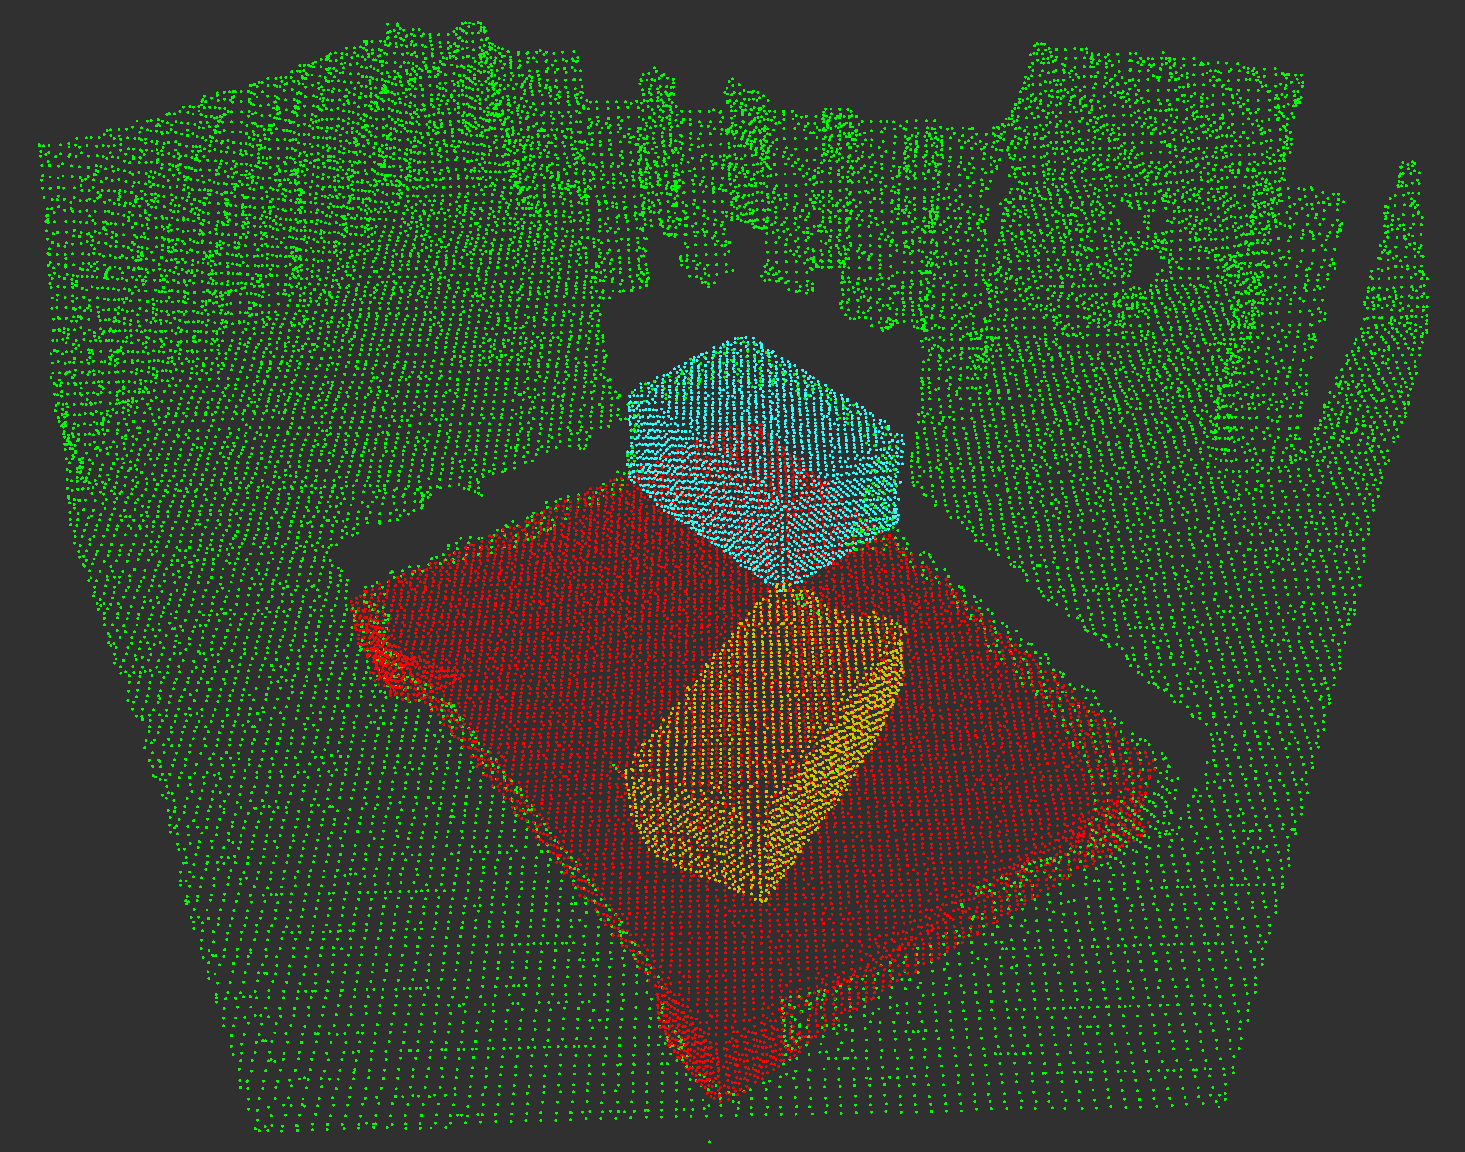
\includegraphics[width = 0.46\linewidth, height=5.0cm]{figs/sample_scene2}
	\label{fig:sample_run}
}
\subfigure[] {
        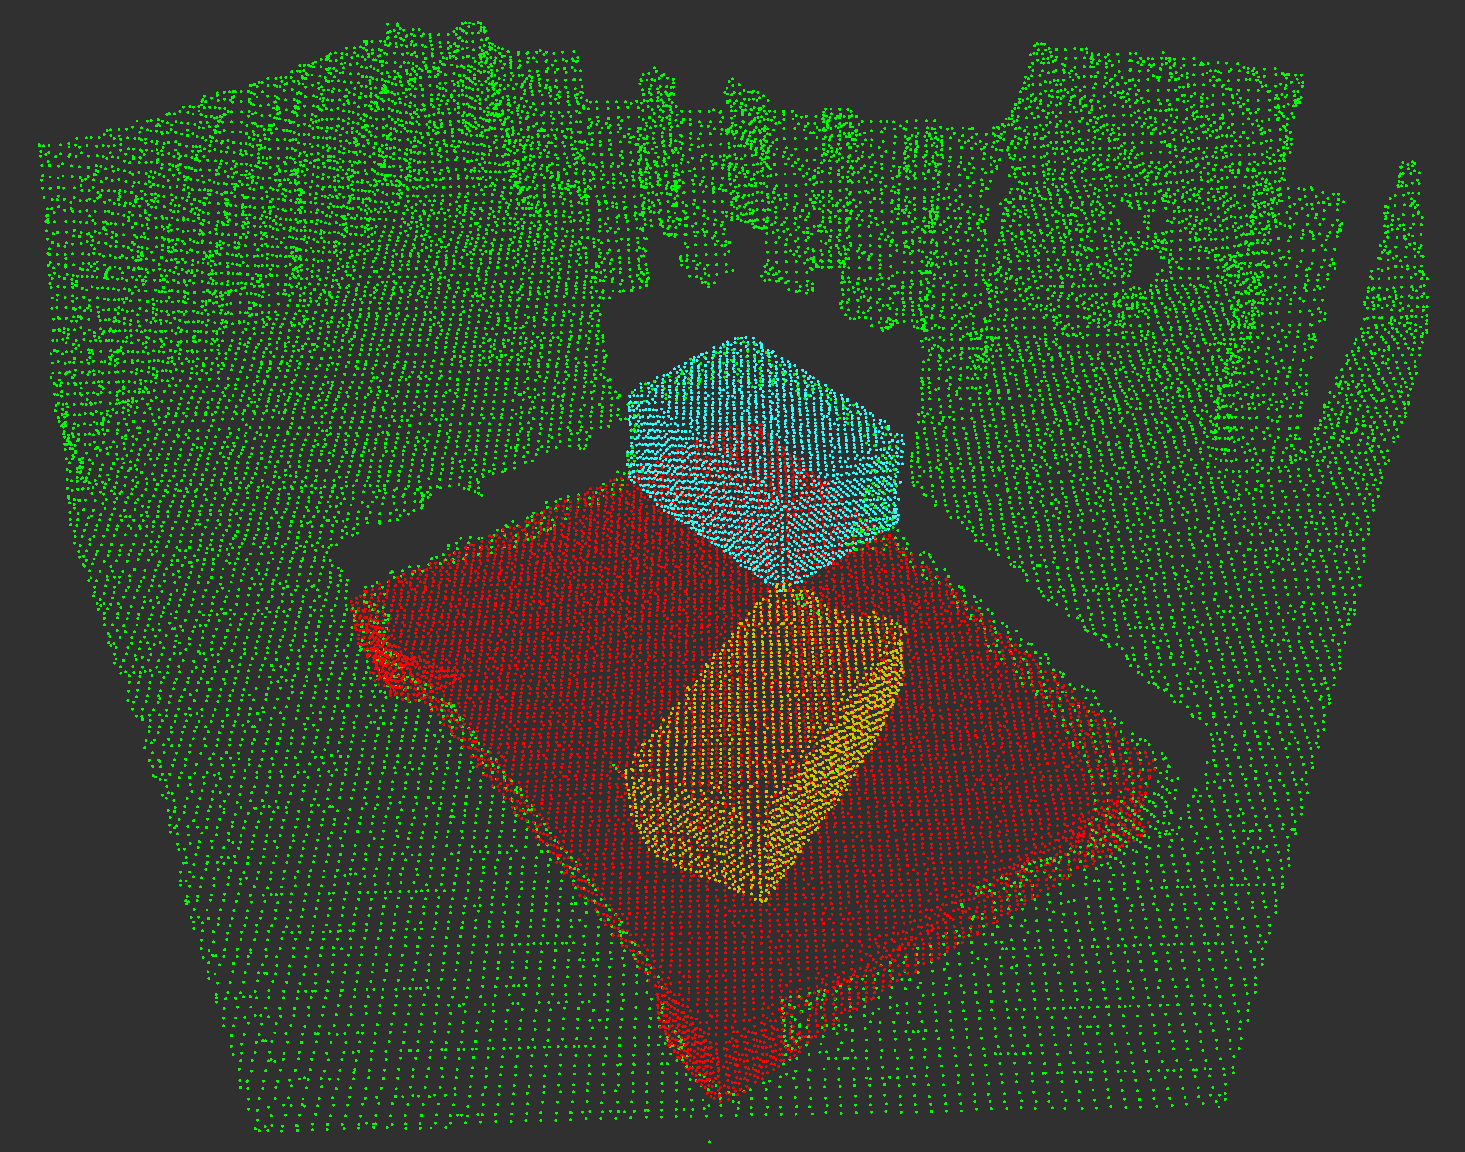
\includegraphics[width = 0.46\linewidth, height=5.0cm]{figs/sample_experiment}
	\label{fig:sample_run_rviz}
}
\caption{Setup used for the experiments in Sec.~\ref{sec:online_evaluation}. A sample scene used in the evaluation is shown in~\subref{fig:sample_run}. A reconstructed test scene model and a corresponding grasp envelope (visualized as a set of selected grasping configurations) are shown in~\subref{fig:sample_run_rviz}.}
\label{fig:tests2}
\end{figure*}
%
%
\renewcommand{\arraystretch}{1.5}
\renewcommand{\tabcolsep}{1.5mm}
\begin{table*}[t!h]
  \caption{Grasp Acquisition Evaluation}
  \vspace{-0.45cm}
  \begin{center}
    \begin{tabular}{l|c|c|c|c|c|c|c|c|c|c}
      Object  & \# of exp. & Success & Rate [\%] & $Q$ & $l \, [rad]$ & $t^p \, [s]$ & $t^e \, [s]$ & $t^m \, [s]$ & $t^g \, [s]$  & $\sum t \, [s]$     \\
      \hline \\ [-3.2ex]
      Duplo  & $20$ & $17$ & $85.0$ & $161.4\pm109.4$ & $4.3 \pm 0.9$ & $14.9 \pm 3.0$ & $0.06 \pm 0.11$ & $25.9 \pm
      3.8$ & $14.7 \pm 3.9$ & $55.6 \pm 5.3$ \\
      Cup    & $16$ & $16$ & $100.0$ & $51.2\pm27.5$ & $4.7 \pm 1.3$ & $13.7 \pm 3.5$ & $0.06 \pm 0.05$ & $10.8 \pm
      0.2$ & $6.9 \pm 2.6$ & $31.5 \pm 3.7$ \\
      Bottle & $17$ & $15$ & $88.2$ & $67.1\pm68.3$ & $4.9 \pm 2.3$ & $14.0 \pm 3.3$ & $0.03 \pm 0.05$ & $10.8 \pm
      0.4$ & $8.5 \pm 3.9$ & $33.3 \pm 6.1$ \\
      Ball   & $20$ & $17$ & $85.0$ & $32.7\pm16.6$ & $5.6 \pm 0.4$ & $13.9 \pm 3.4$ & $0.06 \pm 0.05$ & $10.8 \pm
      1.4$ & $13.9 \pm 4.3$ & $38.7 \pm 4.9$ \\
      Teddy  & $19$ & $12$ & $63.2$ & $28.9\pm13.8$& $5.6 \pm 0.5$ & $15.5 \pm 2.8$ & $0.06 \pm 0.07$ & $10.6 \pm
      0.9$& $11.5 \pm 4.6$ & $37.8 \pm 4.3$ \\
      \hline
      Total & $92$ & $77$ & $83.7$ & $69.46\pm78.06$ & $5.0 \pm 1.3$ & $14.4 \pm 3.2$ & $0.06 \pm 0.07$ & $14.1 \pm
      6.6$ & $11.4 \pm 4.9$ & $39.9 \pm 10.0$\\
    \end{tabular}
    \label{tab:grasp_acquisition}
  \end{center}
 \vspace{-0.25cm}
\end{table*}
%
%
In order to evaluate the usefulness of the extracted envelopes for the purpose of autonomous grasp
acquisition, we also integrated the proposed envelope extraction algorithm into the inequality
Stack-of-Tasks (SoT)~\cite{Kano11} manipulator control framework implementation we presented in~\cite{Krug15}. 
In our experimental setup, we mounted the Velvet Fingers gripper (augmented with an Asus Xtion Pro depth camera) on a KUKA LWR 4+ robot. 
We roughly (by hand) placed one of the target objects shown in Fig.~\ref{fig:setup} at a known picking location, while the other four objects were placed pseudo-randomly in the workspace to simulate clutter (sample scene configuration shown in Fig.~\ref{fig:sample_run}).
The five objects used in these experiments were: a plush teddy bear (Teddy, $82$ g), a stack of
duplo blocks (Duplo, $60$ g), a water bottle (Bottle, $103$ g), a coffee mug (Cup, $134$ g), and a
toy ball (Ball, $54$ g). The two grasp envelope primitives generated in the previous sub-section (at a model resolution of $10$~mm) were used also in this trial: the cylindrical primitive was associated to the Bottle, Cup and Duplo objects, while the spherical one was used for the Teddy and Ball objects. 
%
\par
In each experimental run we first controlled the manipulator to move the gripper-mounted camera to three pre-defined scene observation poses.
Simultaneously we built a TSDF model from the depth images, using camera poses obtained through the robot's forward kinematic model. 
We then used our grasp envelope extraction procedure to obtain constraints on the gripper posture
for the target object, which were subsequently used to form control tasks used in the SoT framework (see~\cite{Krug15} for a more in-depth description).
At this point, we made a slight modification to the envelope extraction procedure in order to obtain
envelopes that were more likely to be reachable for the employed robot arm. 
To this end, we imposed additional constraints on the gripper orientation prior to extracting the
grasping envelopes, requiring the final end effector orientation to be within a cone of width $\frac{\pi}{2}$~rad, centered at the initial end effector orientation.
A sample grasp envelope extracted in this manner from a training scene is shown in Fig.~\ref{fig:sample_run_rviz}.
Once the manipulator motion control satisfied the grasp envelope constraints, we executed the grasp
acquisition routine described in~\cite{Krug14a}, in order to obtain an enveloping grasp of the target object.
A trial was judged successful if the target object could be lifted and extracted from the scene. 
We performed twenty trials for each target object, with varying placement poses of the surrounding objects in the scene.
\par
The results of this set of experiments are summarized in Table~\ref{tab:grasp_acquisition}.
For each of the test objects we report respectively: 
the number of experiments performed; 
the number of successful grasps; 
the respective success rate; 
the grasp envelope quality $Q$; 
the trajectory length $l=\int_0^{t^m}\norm{\dot{\mbm{q}}(t)}_1dt$ as the sum of angular distances traveled by all joints of the manipulator; 
the times $t^p$, $t^e$, $t^m$, and $t^g$ for the pre-positioning, envelope extraction, grasp pose
approach motion and grasp acquisition phases respectively; 
as well as the total time for each run $\sum t$.  
In eight of the trials the target object was occluded from the sensor view point and our approach did not find a suitable grasping envelope. 
These trials are excluded from the statistics in Table~\ref{tab:grasp_acquisition}.
\par
The obtained statistics are relatively uniform across the different trials and different objects, with two minor exceptions.
First, the success rates for the Teddy are notably lower than for the rest of the target objects.
This discrepancy is unlikely to be linked to the size of the extracted envelopes, which are almost on par with the other object associated to a spherical envelope primitive (the Ball).
We attribute the lower success rate chiefly to the lower friction coefficient of the Teddy, which leads to frequent slippage against the belts of the Velvet Fingers gripper and consequently a lower likelihood of attaining a stable grasp. 
The second discrepancy is in the substantially longer trajectory execution times ($t^m$) for the Duplo object. 
The reason for this is that the underlying task dynamics parameters in the SoT framework were adjusted after the tests on the Duplo object, in order to speed up testing.
We also note the reasons for failure in grasping for the remaining objects: for the Duplo object, two failures were due to the object toppling over and one failure was due to a collision with an obstacle during approach; for the Bottle, both failures were due to the object toppling; finally, for the Ball all three failures were due to the object rolling out of the gripper upon contact. 
Finally, the grasp envelope extraction procedure produced slightly smaller volumes in comparison to the offline tests from Sec.~\ref{sec:offline_tests}, due to the additional constraint on end effector orientation. 
The reported envelope extraction run-times $t^e$ were consistent, allowing for some overhead for message passing between different nodes.
%

%
\section{Discussion}
\label{sec:discussion}
%
In this article we propose a method for extracting grasp envelopes --- constraints on gripper pose and joint configurations --- from online reconstructed workspace models.
We utilize knowledge of basic human grasping strategies to define two grasp envelope primitives favoring grasps along the target object PCA directions. 
\par
A limitation of the current work is the lack of rigorous treatment of kinematic feasibility of the extracted envelopes.
Therefore, we plan to extend our approach using information of the likelihood of achieving grasp poses, $e.g.$ by using capability maps~\cite{Zach07}.
%
\bibliographystyle{IEEEtran}
\bibliography{References}

\end{document}



